\chapter{Evolution of system design}
\label{chap:evolution}

To track sleep unobtrusively, multiple techniques and sensor types have been tested and evaluated by other researchers. Placing load cells under the bed supports allowed researchers to determine the precise time when subject fell asleep and when subject woke up\cite{load_cells}. Infrared camera recording of subjects sleeping allowed precise recognition of small movements even under the blanket \cite{video}. Another research group used \ac{POF} sensors to recognize breathing patterns and detect apnea\cite{optical}. The same results were also achieved using pneumatic pressure sensors placed in a sealed air-cushion under the mattress\cite{pneumatic}. In yet another research, a group of researchers conducted experiment in which they placed two $24 GHz$ radars under the bed and found out that it is possible to accurately recognize hearth rate\cite{radar}.

But, one of the recently most popular methods of unobtrusive sleep tracking is much simpler and more affordable than the others. It is called pressure sensing and it involves continuous measurement of pressure from under the subject. This thesis picks up on the work of Prof. Dr. Ralf Seepold, Ra\'ina Kuhn, Daniel Scherz and Maxime Guyot at \ac{UC-Lab}\cite{Kuhn}\cite{Guyot} who have successfully used pressure sensors to determine position, detect movement and track vital signs during sleep.


\section{Devices and technology}

To achieve a good sleep tracking from pressure readings under the bed, an appropriate environment has to be selected. Environment consists of an adequate bed frame, a mattress and of base-plates which hold the mattress in the frame of the bed. Bed frame is of a regular size - $90 * 200cm$ which accommodates vast majority of people. Because of good pressure propagation, mattress should not be too firm or too tight. Therefore, mattress of uniform hardness level 2 has been selected.

To hold the mattress in place, a grid of pressure-disks is used. They are critical part of the system as they have to absorb the pressure from the mattress. Also, they are the point at which pressure measurement can be done. To provide a better granularity, pressure-disks provided by ErgoProTech and depicted in Figure \ref{fig:base-plate} were used. They were placed 3cm from each other under the whole area of the mattress according to the manufacturers usage recommendation. This ensures adequate support across the mattress. For selected mattress size, base-plate grid consists of 12 rows and 5 columns totaling in 60 pressure-disks. Pressure-disks are made of semi-elastic polymer and consist of 4 connected rectangular blades. These blades are supported by 4 double arms anchored at the same point where the whole structure is connected to the bed frame. There are multiple hardness levels of base plates and they are differentiated by the color of the rectangular blades. Firmer base plates are grey while more elastic ones are purple. More about placement of pressure-disks can be found in \autoref{ssec:test_environment}

\begin{figure}[h]
  \begin{center}
    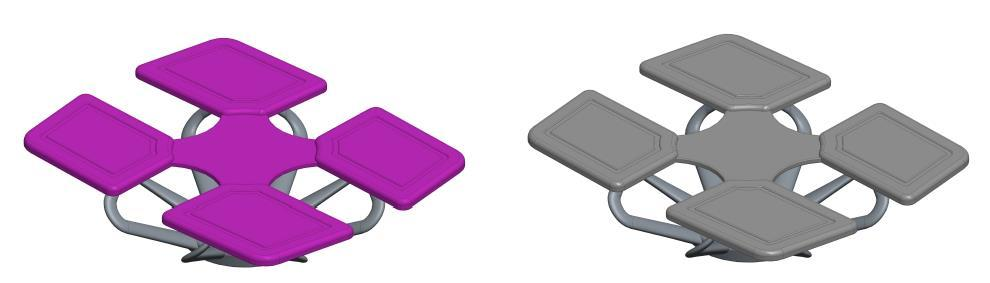
\includegraphics[width=0.5\linewidth]{1-base_plate.jpg}
  \end{center}
  \caption{Base plates in the bed.}
  \label{fig:base-plate}
\end{figure}

There are multiple types of pressure sensors that could be used for the purpose of this project\cite{pressure_sensors}. Potentiometric pressure sensors are very crude due to their construction and often have reliability and hysteresis issues. Inductive pressure sensors require \ac{AC} excitation of coils and consequentially signal filtering and demodulation. Piezoelectric and piezoresistive pressure sensors measure change of pressure using piezoelectric effect. Capacitive pressure sensors use a small diaphragm as a capacitor plate. When pressure is applied, diaphragm deflects and capacitance changes. Change may or may not be linear and usually is on the order of a few $pF$ while total capacitance of the sensor is between $50$ and $100 pF$ which means that it may be hard to precisely measure the values. This method may also suffer from environmental effects and inadequate \ac{PCB} or protoboard design decisions. \ac{FSR} is a type of material whose resistance changes when a pressure is applied. Advantages of \ac{FSR} sensors over other pressure sensors are possibility of detecting static pressure, its flexibility, thinness and inexpensiveness. Multiple other researches were made using the same type of sensor and have proven its reliability and accuracy when used in a sensor grid\cite{pillow_system_1}\cite{pillow_system_2}\cite{apnea_low_cost}. Therefore, this type of sensor was selected for use in this specific project.

So how does the \ac{FSR} sensor work? \ac{FSR} is a \ac{PTF} device which exhibits a decrease in resistance with an increase of the force applied to the active surface\cite{fsr_guide}. At 'zero force', conductive ink is separated from the active area by spacer adhesive and in that case \ac{FSR} sensor has the highest possible resistance. When pressure is applied to sensor, conductive layer is pushed down onto the active area which results in a decrease of resistance. Construction of FSR sensor is shown in Figure \ref{fig:fsr-sensor}. For a hemispherical sensor with a diameter of 12.7mm (model 402) sensibility starts just below $20 g$ and extends to around $10 kg$ when saturation occurs. Passing a threshold at around $20 g$, resistance changes from greater than $100 k\Omega$ to $10 k\Omega$. After that resistance falls logarithmically with an increase of force as seen in Figure \ref{fig:fsr-sensor}. For consistent results application manual\cite{fsr_guide} suggests using a firm, flat and smooth mounting surface and use of a rubber spring to spread the pressure over the whole sensitive area. Also, an appropriate sensor size and shape is to be used.

\begin{figure}[h]
  \begin{center}
    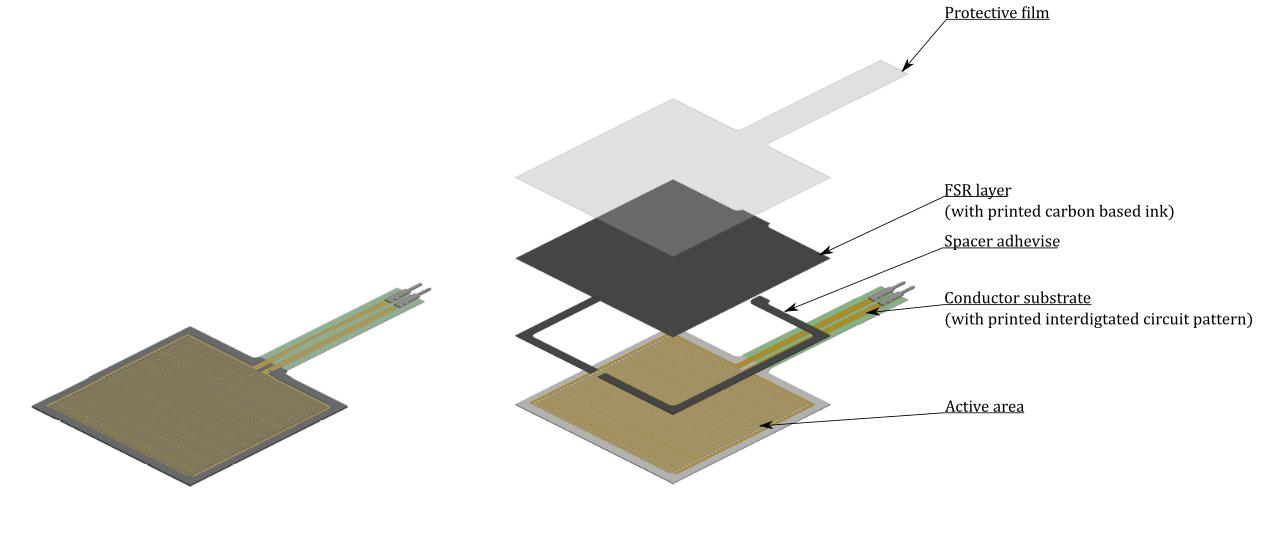
\includegraphics[width=0.50\linewidth]{1-fsr_sensor.png}
    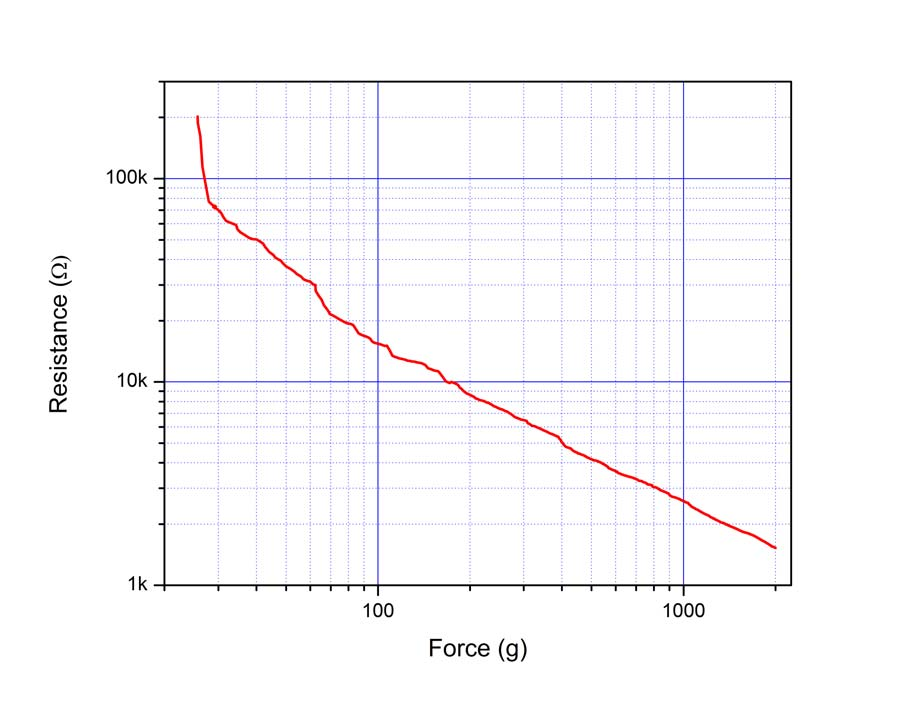
\includegraphics[width=0.33\linewidth]{1-fsr_graph.png}
  \end{center}
  \caption{FSR sensor construction and resistance characteristics.}
  \label{fig:fsr-sensor}
\end{figure}

There are 4 different types of standard of-the-shelf sensors\cite{fsr_guide} and their sizes and shapes are shown in Table \ref{tab:fsr_types}. Models 400 and 402 also have short-tailed variants which feature shorter connection between \ac{FSR} pads and pins found at the end of the lead wires. These same models have a small pressure sensing surface and are not as well suitable for this project. Models 406 and 408 have much larger contact surface area, which means that a more consistent distribution of pressure is possible. Model 406 is perfect for use in areas that require good position resolution such as scapular area. On the other hand, type 408 can be used in crural region.

\begin{table}[h]
  \begin{center}
    \begin{tabular}[h]{ | >{\centering\arraybackslash} m{3cm} | >{\centering\arraybackslash} m{3cm} | >{\centering\arraybackslash} m{7cm} | }
      \hline
      Part number & Description & Part image \\ 
      \hline
      Model 400 & 0,2" circle & 
\includegraphics[height=1.3cm]{1-fsr_400.png} \\  
      Model 402 & 0.5" circle & 
\includegraphics[height=1.3cm]{1-fsr_402.png} \\
      Model 406 & 1.5" square & 
\includegraphics[height=1.3cm]{1-fsr_406.png} \\  
      Model 408 & 24" strip & 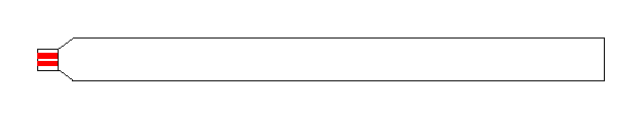
\includegraphics[height=1.3cm]{1-fsr_408.png} \\
      \hline
    \end{tabular}
  \end{center}
  \caption{Standard shapes and sizes of FSR sensors offered by Interlink Electronics.}
  \label{tab:fsr_types}
\end{table}

To get a reading of sensor resistance ($R_{fsr}$), a sensor is connected in a series with a fixed value reference resistor ($R_{ref}$). Then, an input voltage ($V$) is applied to the circuit. Voltage drop ($V_{fsr}$) is measured on the \ac{FSR} sensor leads. Pressure applied to sensor is in a reciprocal correlation to the $R_{fsr}$ because \ac{FSR} has a maximal resistance when there is no external force pressuring its surface as seen in Figure \ref{fig:fsr-sensor}. The same graph is also sampled for force-resistance pairs which are used for reference resistor selection. $R_{fsr}$ needs to be selected in such a way that it has best resolution for force between $0 kg$ and $1.6 kg$. These weight values were selected based on R. Kuhns calculation\cite{Kuhn}. She took an average weight of a person and mattress and calculated an estimate of how much weight each of the disk springs carry. Equation \ref{eq:fsr-calculation} describes the relation between $V_{fsr}$ and $R_{fsr}$ when a $R_{ref}$ has a fixed value. Multiple standard resistor values were put into the equation and at resistance of $10 k\Omega$ change gradient was highest. Therefore, $10 k\Omega$ resistor was used as $R_{ref}$.

\begin{figure}[h]
  \begin{equation}
    \label{eq:fsr-calculation}
    V_{fsr} = \frac{V*R_{ref}}{R_{fsr}+R_{ref}}
  \end{equation}
\end{figure}

Initial sensitivity tests that were conducted by R. Kuhn and M. Guyot showed that additional layer should be added on top of the \ac{FSR} sensors to help with pressure absorption. In Figure \ref{fig:fsr-sensor} it is clearly visible that adhesive spacer layer creates a non-sensitive frame around the active sensor area. When sensor surface was directly exposed to the mattress, adhesive absorbed most of the pressure as it was not as elastic as active area. This was solved by using felt\footnote{textile material that is produced by matting, condensing and pressing fibers together.} gliders. This greatly improved the sensitivity and results can be seen in Figure \ref{fig:felt_gliders}.

\begin{figure}[h]
  \begin{center}
    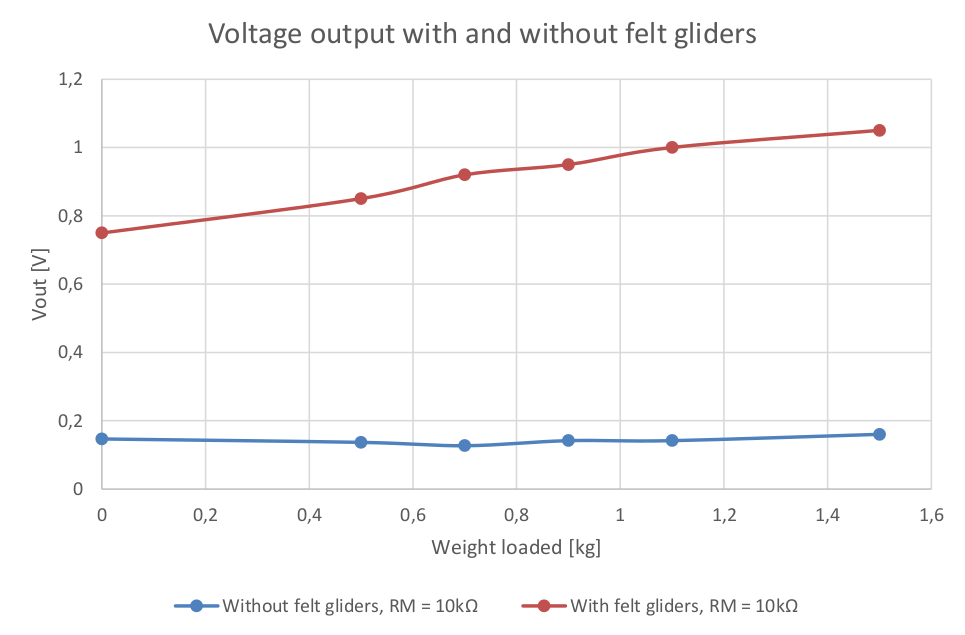
\includegraphics[width=0.7\linewidth]{1-felt_gliders.jpg}
  \end{center}
  \caption{Comparison of pressure with and without felt gliders.}
  \label{fig:felt_gliders}
\end{figure}

To convert voltage to a digital value, \ac{ADC} was done with a help of a microcontroller. Sensors were connected to the Trinket Pro 5V microcontroller development board\cite{Trinket}. This board features ATMega328P microcontroller with integrated \ac{ADC} functionality\cite{atmega328p}. From a myriad of different boards this one was chosen because it can be programmed as Arduino Pro Mini but features 8 analog input pins. Unfortunately, two of the analog pins share functionality with \ac{I2C} protocol and 1 was used for board identification. This means that 1 board could support up to 5 sensors. To collect readings from multiple devices, already mentioned \ac{I2C} protocol was used. A device that takes readings from the pressure sensors and can communicate with the rest of the system will be called a node in the rest of the thesis.

But it would be quite impractical to connect a \ac{PC} to each an every node to collect data. So the system was designed with a new device as an endpoint. This device communicates as \ac{I2C} master with the nodes and allows easier communication between user and the nodes. For purpose of an endpoint, Intel Edison \ac{COM} was used. It features Intel Atom \ac{CPU} and Intel Quark 32-bit microcontroller\cite{Edison}. Both have x86 architecture and use x86 instruction set. But what is more important, Intel Edison has $4GB$ \ac{EMMC} storage as well as integrated \textit{Bluetooth} and \textit{Wi-Fi}. Using Wi-Fi, sensor readings paired with their position were transmitted to locally situated web server. Web server application saved the incoming data into the database and provided \ac{API} for the client application. Using client application, user was able to calibrate and review sensor data.


\section{Test environment}
\label{ssec:test_environment}

To get a better result recognizing sleep position, a sleeping recognition sensor network has to be designed in such a way that it is able to detect all of the most common sleep positions. Figure \ref{fig:sleep_positions} shows 6 positions people most often sleep in. From left to right those are fetal position, log position, yearner position, supine position, starfish position and prone position. Fetal, yearner and log position can be left or right depending on the bed side subject is facing. But since there is no difference in weight distribution between left and right log position, it is possible just to classify position as log position. This means that total of 8 different positions can be classified using pressure sensing. Using commercial pressure sensing mat and pattern matching, a research conducted in a clinic has achieved 97\% classification accuracy\cite{postures} which means that this technique is very reliable. But, putting a \ac{FSR} sensor pad on every possible blade would require 240 sensors and 48 nodes which is not only expensive in terms of hardware cost but also of time used for setting up the system. The easiest way to minimize the complexity would be reducing the number of sensors but it has to be done in such a way that there is no significant classification accuracy loss compared to fully populated base-plate area. Since vertical movement during sleep is rare and all of the major body regions exceed the surface area of a sensor, the emphasis was placed on horizontal resolution. Pressure sensors were placed on two blades in the same row while the other row was left without sensors. This decision reduced the number of required sensors from 240 to 120.

\begin{figure}[h]
  \begin{center}
    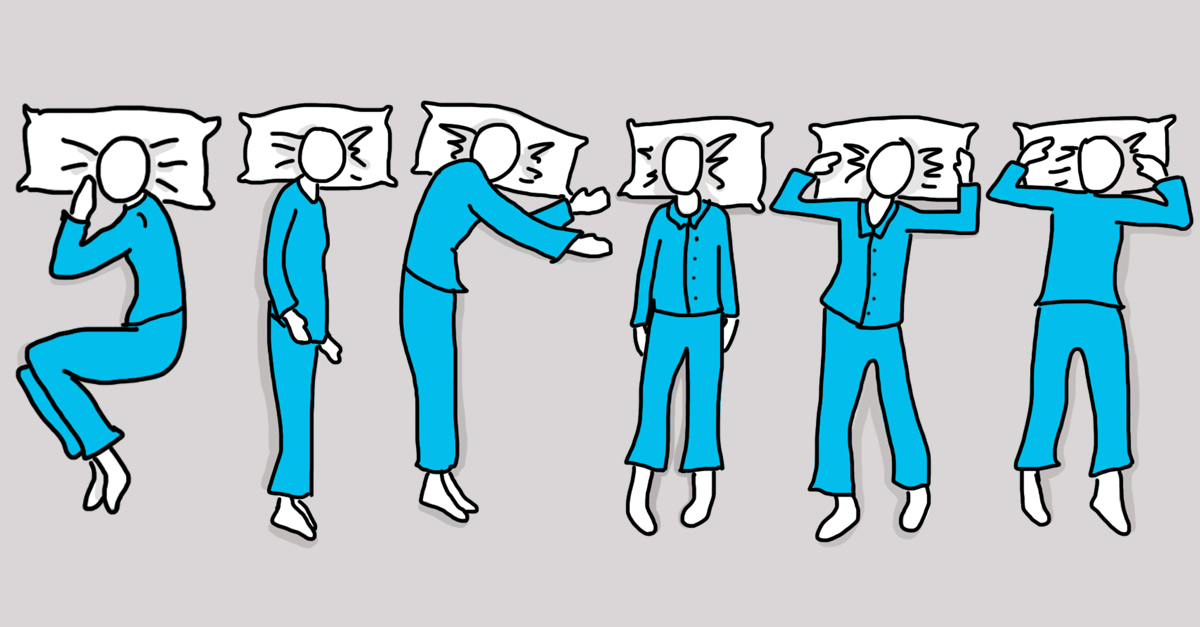
\includegraphics[width=0.4\linewidth]{1-sleep_positions.jpg}
  \end{center}
  \caption{Different sleep positions.}
  \label{fig:sleep_positions}
\end{figure}

To retain the possibility of accurate position recognition but to further minimize the number of sensors used, a look was taken into the weight distribution during supine and log position. In Figure \ref{fig:sensor-layout} we can see that mattress deflects the most in scapular, gluteal and crural regions. Scapular area is especially important because it is the area where respiration and heart rate detection is done. Other areas of the body are not as important to create an accurate picture of the body position and to measure vital signs. Also, at the edge of the bed frame, mattress is transferring a significant amount of pressure to the frame which means that these pads are not very sensitive. As a conclusion, 48 sensors were placed in 6 rows as seen in Figure \ref{fig:sensor-layout} and according to M. Guyots\cite{Guyot} sensor layout proposal.

\begin{figure}[h]
  \begin{center}
    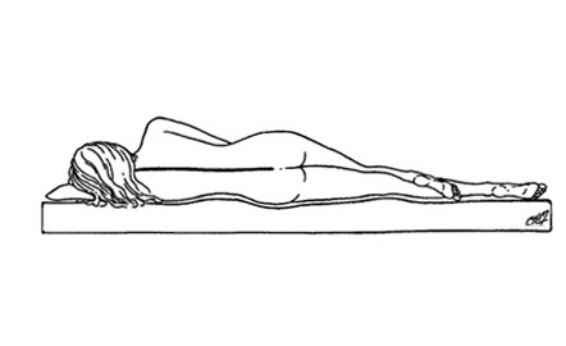
\includegraphics[width=0.4\linewidth]{1-weight_distribution.png}
    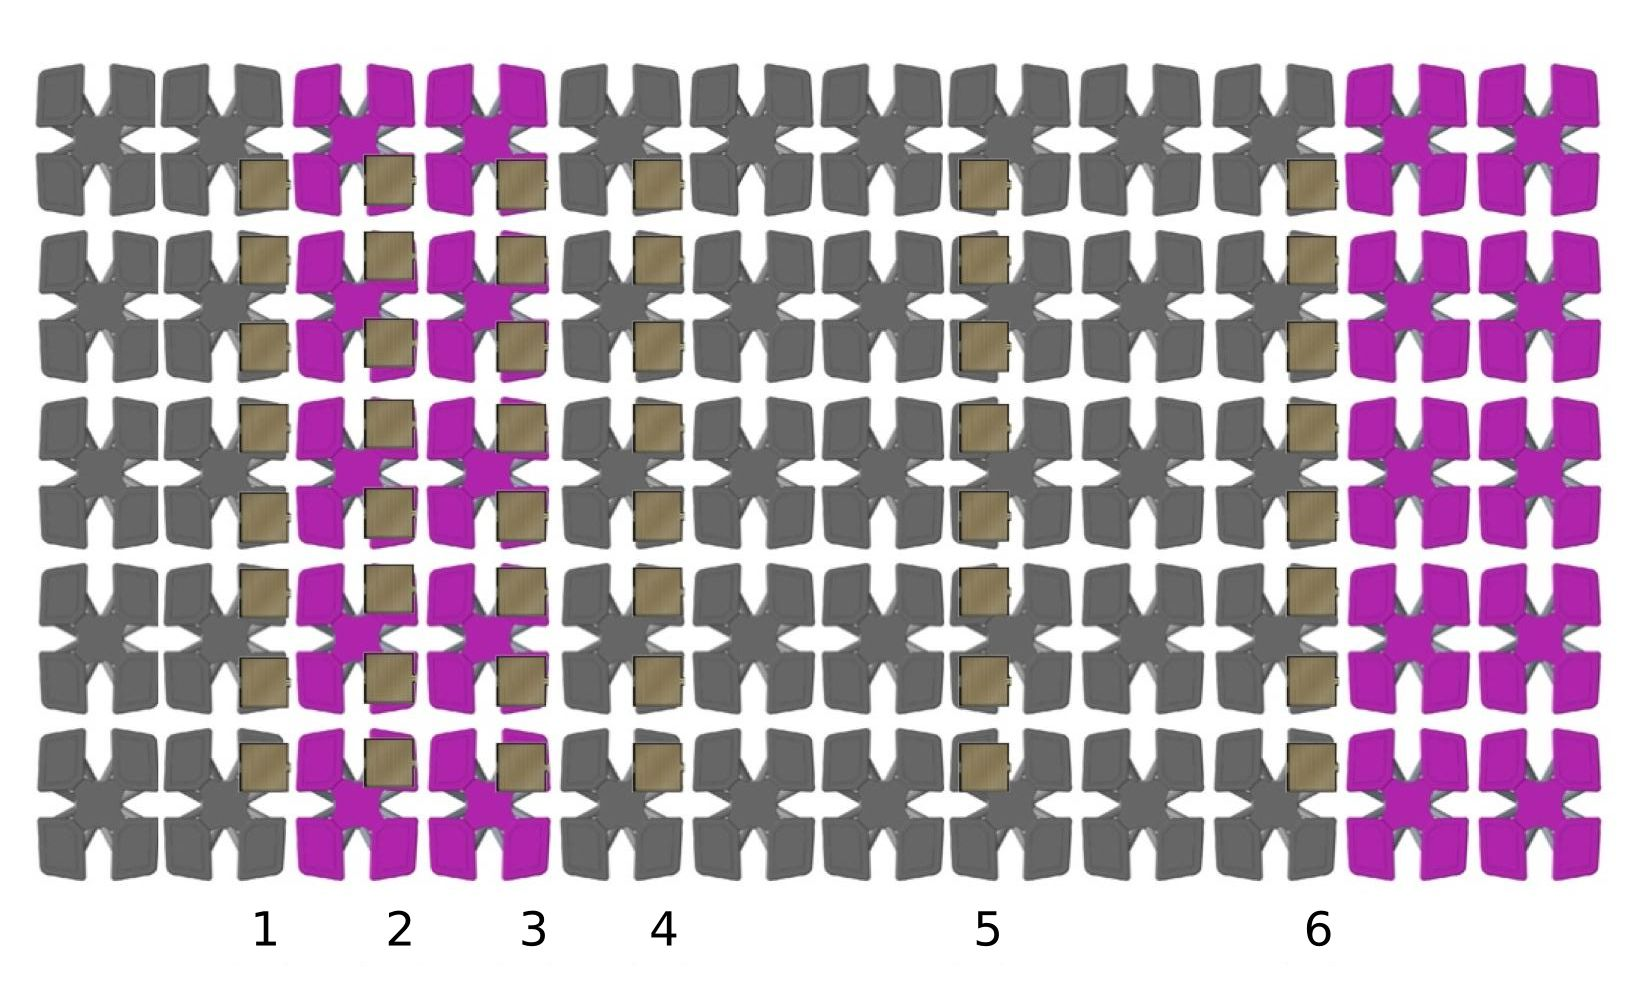
\includegraphics[width=0.4\linewidth]{1-sensor_layout.jpg}
  \end{center}
  \caption{Sensor arrangement in bed compared to sleep position.}
  \label{fig:sensor-layout}
\end{figure}

The described system with 48 sensors required 10 Trinket Pro boards. As all of the boards were communicating using \ac{I2C} protocol in which each of the slaves has a unique address, addresses had to be distributed in accordance with their physical position. This required either a different firmware for every board or some smarter alternative in which every board would automatically select different I2C address in an orderly way. The solution that was proposed involved using same-value resistors in a series. Depending on the voltage difference between identification resistor and ground, an \ac{I2C} address was chosen by the microcontroller. Although this solution was easy to implement, it had used up one ADC pin that could have been used for sensor connection. Since Trinket Pro does not have prototyping holes, 5 reference resistors for sensor reading and 1 for position identification had to be added. For every reference resistor a perforated electronic prototyping board was cut and a resistor and 3 wires were soldered. Also, position identification resistor was soldered onto a piece of perforated board and connected between two adjacent Trinkets. This means that adding a new node with 5 sensors to the system required 6 new small boards to be soldered. Wiring was something that could have been improved with introduction of a signal bus.


\section{A new architecture}

To address this hardware shortcomings, a new hardware architecture was proposed. In it, sensor nodes were implemented as \ac{PCB}s which featured all previously additionally soldered resistors. A new method of node position identification was developed without the use of identification resistor and connection between nodes was implemented using standardized connectors and cables. This means that \ac{FSR} sensors can now be directly connected to the nodes. Proposed solution eliminated a need for perforated boards and use of soldering iron for installation. The total number of nodes was also reduced to a third by using microcontrollers with more \ac{ADC} inputs. This was done to reduce system cost, power consumption and to make installation and modification of development much simpler.

Endpoint was reimagined to integrate data storage and server functionality so no external servers are now needed for a system to serve data to the client. Web based user interface was also implemented on the endpoint so that results could be viewed from a \ac{PC} or even from a mobile device. But what if there is a need for a service which monitors multiple beds at the same time such as in case of hospital or nursing home? Well, endpoint also serves data over well described API and allows easy readout of data collected from sensor network. A graph depicting a new system architecture is found in Figure \ref{fig:sys_architecture}.

\begin{figure}[h]
  \begin{center}
    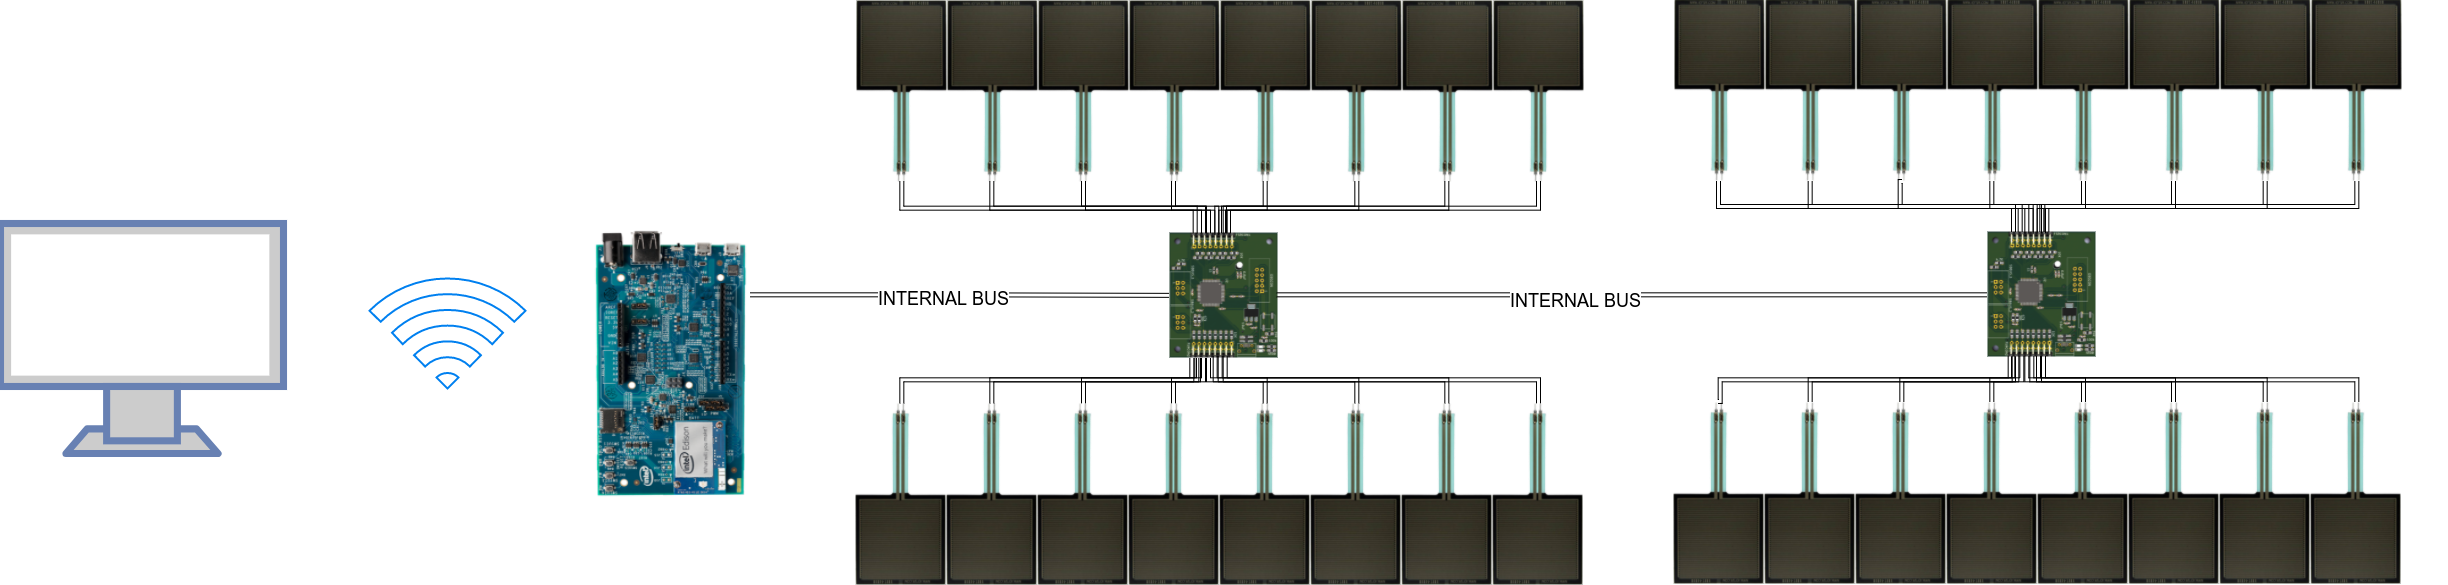
\includegraphics[width=\linewidth]{1-hardware_system_design.png}
  \end{center}
  \caption{A newly implemented system architecture.}
  \label{fig:sys_architecture}
\end{figure}